A basic obstruction-free queue is given in Listing \ref{lst:queue}. From this
queue, the authors construct a wait-free queue by using the fast-path-slow-path
methodology.

$FAA(x, v)$ atomically reads the value stored in the $x$ variable, and
increments it by $v$. $CAS(x, t, v)$ atomically reads the value stored in $x$,
compares it to $t$ and, if $x$ is equal to $t$ (success), replaces the value of
$x$ by $v$. $CAS$ returns whether it has successfully replaced the value or not.

\begin{lstlisting}[mathescape,
                   frame=single,
                   caption={An obstruction-free queue using an infinite array.},
                   label={lst:queue},
                   language=C]
Q: queue
T: pointer to tail
H: pointer to head
enqueue(x: var) {
  do t := FAA(&T, 1);
  while (!CAS(&Q[t], $\bot$, x));
}
dequeue(x: var) {
  do h := FAA(&H, 1);
  while (!CAS(&Q[h], $\bot$, $\top$) and T > h);
  return (Q[h] == T ? EMPTY : Q[h]);
}
\end{lstlisting}

\para{Basic queue} This queue uses a shared (emulated) infinite array to
store elements. We will see later how this is done and how memory can be
reclaimed. Two special values are reserved : $\bot$ (bottom) and $\top$ (top).
$\bot$ stands for empty cells as the queue is initially filled with $\bot$.
$\top$ stands for unusable cells. When one thread dequeues an element, he marks
the cells with $\top$ to prevent other threads to enqueue an element in it.

To enqueue an element, one thread try to find an available cell on the array, a
cell marked with $\bot$. One cannot enqueue an element in a $\top$ marked cell
because it could violate the FIFO property of the queue. To get an unique index
on the array, they uses fetch-and-add to increment the shared tail pointer.
Considering the pointer is shared by all threads, using compare-and-swap instead
of fetch-and-add would result in lots of failures. After one thread is given an
unique index, he needs to certify that the cell is empty. He then uses
compared-and-swap to enqueue an element into the array. In case of
compare-and-swap failure, redo the whole process until the element is enqueued.

The dequeue operation works in a similar manner, one thread try to find either a
cell filled with an element or marked with $\top$ by using fetch-and-add on a
shared head pointer. If a thread stops on a $\top$ marked cell, the dequeue
returns \texttt{EMPTY}.

This queue is designed to be fast. Dequeue may always fail if queued values are
dequeued by another thread. Enqueue may always fail if another thread mark each
empty cell unusable. As a result, it is neither wait-free or lock-free because
it is proned to livelocking. As only one thread is guaranteed to progress, this
queue is only obstruction-free. \\

\begin{figure}
    \caption{The fast-path-slow-path methodology \cite{Kogan:2012:MCF:2370036.2145835}.}
    \label{fig:fpsp}
    \center
    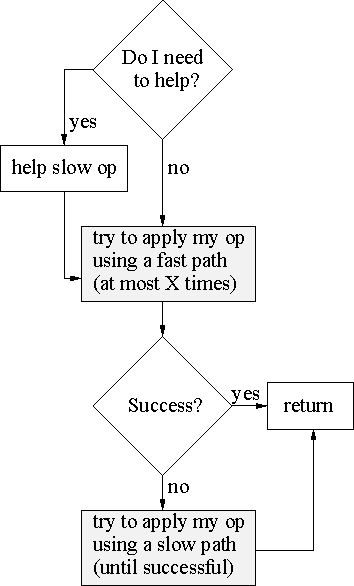
\includegraphics[width=0.6\linewidth]{img/fpsp.pdf}
\end{figure}

\para{Fast-path-slow-path} To construct a wait-free realization of the previous
queue, the authors use the fast-path-slow-path methodology. As shown in figure
\ref{fig:fpsp}, one thread tries to enqueue or dequeue an element using a
fast-path, which is similar to the previous queue. A maximum number of failures
is set. If a thread failed too many times to apply his operation, he falls back
on a slow-path.

For example, if a thread fails to enqueue an element, he publishes an enqueue
request. When others threads want to dequeue an element, they look at all
pending enqueue requests, and eventually help one request to complete. The
enqueuer thread then keeps trying to enqueue the element until he or another
succeeds.

Threads are linked in a ring, they keep a pointer to a \textit{peer} to who they
help operation to complete. Each time a thread successfully helps another
thread, he updates his \textit{peer} to the next thread in the ring so that each
thread happens to help every one at some point. \\

\para{Memory reclamation} The authors designed their queue with an infinite
array. To do so, the queue is split into segments as a linked list. Each segment
contains a fixed number of cells. The list of segments is expanded as necessary.
Because the tail and head pointers are never decremented, segments no longer in
use needs to be freed.

After one thread dequeues an element, the thread tries to reclaim memory from
unused segments. They uses compare-and-swap to achieve mutual exclusion so that
if several threads try to reclaim memory, only one should succeed. Unused
segments are segments filled with $\top$ marked cells. The \textit{cleaner}
thread ensures no threads keep a reference to a segment about to be freed.

overhead \\

\para{Wait-free guaranty}
idée de preuve wait-free et linearizable
